\documentclass[11pt]{article}
\usepackage[T1]{fontenc}
\usepackage{mathpazo}
\usepackage[scaled=0.92]{helvet}
\usepackage{courier}
\usepackage[margin=1in]{geometry}
\usepackage{amsmath,amssymb}
\usepackage{booktabs,threeparttable,array}
\usepackage{graphicx}
\usepackage[font=small,labelfont=bf]{caption}
\usepackage[expansion=false]{microtype}
\usepackage[colorlinks=true,linkcolor=blue!50!black,citecolor=blue!50!black,urlcolor=blue!50!black,pdfstartview=FitH]{hyperref}
\usepackage{xcolor}
\graphicspath{{figures/}}
\newcommand{\fpd}{\textsf{fp64}}
\newcommand{\fps}{\textsf{fp32}}
\setlength{\tabcolsep}{4pt}
\makeatletter\let\tabinput\@@input\makeatother

\title{The Diffusion Model of Partial Default in CUDA and C++:\\ Performance, Single Precision, and Dense Grids}
\author{Grok Bot}
\date{November 2026}

\emergencystretch=3em
\begin{document}
\maketitle

\begin{abstract}
\noindent This report describes a performance-oriented rewrite of the main computation of the quantitative diffusion model of partial default: the equilibrium of the main calibration, its ergodic distribution, the simulated and ergodic moments of Table~2, and the impulse responses of Figure~8 and Figure~F.1. The rewrite is one C++/CUDA code with a multicore CPU back end and a GPU back end, each templated on the floating-point type. On the paper's $201\times75$ grid the full pipeline runs in 0.54 seconds on the GPU in single precision and in 1.2 seconds on the CPU in double precision, against 20 seconds for the paper's code, and the double-precision solution agrees with the paper's code to the solver tolerances. The same code solves the model, with its simulation and impulse responses, on a $500\times121$ grid in 2.1 seconds and on grids of $1000\times121$ and $2000\times121$ in 3.1 and 5.6 seconds on the GPU. Single precision converges under a precision-scaled stopping rule and reproduces the double-precision moments to the reported digits.
\end{abstract}

\tableofcontents

\section{Scope and hardware}

The computation is the main calibration of the diffusion model: the parameter vector stored with the replication package (\texttt{data/ou\_main.npz}), solved from the package's starting point (\texttt{data/calibration/start.npz}) with the solver settings and strict tolerances of the package's confirmation step (\texttt{cal\_core.SOLVER} and \texttt{STRICT}). Each run produces four stages:
\begin{enumerate}
\item \emph{Solve}: the equilibrium value $V(B,z)$, price $q(B,z)$, consumption $c$, default intensity $d$, and drift of debt $S$ on a grid of $n_B$ debt levels on $[0,1]$ and $n_z$ log-endowment levels on $\pm2.5$ stationary standard deviations.
\item \emph{Ergodic}: the ergodic density $g(B,z)$, the null vector of the transposed generator.
\item \emph{Moments}: the ergodic moments and the moments of 16 simulated paths of 25{,}000 years with 100 steps a year, which together give Table~2 and the calibration loss.
\item \emph{IRF}: the expected paths after a shock of $-0.1$ to $z$ from the ergodic distribution (Figure~8) and from three states (Figure~F.1), by the forward equation over 21 years.
\end{enumerate}
Recalibration and robustness checks are outside the scope.

The machine is a workstation with a 12th-generation Intel Core i7-12700 (8 performance and 4 efficiency cores, 20 hardware threads) and an NVIDIA T1000 8\,GB (Turing, 14 streaming multiprocessors, 896 CUDA cores). The T1000 executes double-precision arithmetic at 1/32 of its single-precision rate, so on this card single precision is the natural GPU precision, and double precision is the natural CPU precision. The code is built with \texttt{nvcc} from the NVIDIA HPC SDK~26.3 (CUDA~13.1, \texttt{-O3}, \texttt{sm\_75}) and GCC~13.3 as the host compiler (\texttt{-O3 -march=native -fopenmp}). The paper's code is Python~3.12 with NumPy, SciPy, and Numba, with Numba's compilation cached before timing.

\section{The equilibrium and the paper's algorithm}

The value function solves a Hamilton--Jacobi--Bellman equation in which the sovereign chooses consumption, issuance, and the default intensity, and the endowment follows an Ornstein--Uhlenbeck process; the price solves a linear pricing equation given the default intensity and the drift of debt. The paper discretizes both equations with an upwind scheme: the drift of debt picks a forward difference, a backward difference, or zero drift at each node (the three \emph{branches}), and the endowment process is a tridiagonal generator in $z$. The equilibrium is the fixed point of implicit pseudo-time stepping. At step $k$, with $(V^k,q^k)$,
\begin{enumerate}
\item the \emph{policy step} computes, at every node and for each branch, the best issuance and default intensity by golden-section search (28 iterations), and keeps the branch with the highest Hamiltonian; a node keeps its branch from the previous step unless another branch beats it by more than $10^{-6}$ (stickiness), and a node whose branch changes three times within 30 steps, once the time step has reached its maximum, keeps its branch from then on (freezing);
\item the \emph{linear step} solves two sparse systems with the generator $A^k$ of the policies:
\begin{align*}
\left[(\rho + \tfrac1{\Delta t_k}) I - A^k\right] V^{k+1} &= u^k + \tfrac{1}{\Delta t_k} V^k, \\
\left[\mathrm{diag}(\xi^k + \tfrac1{\Delta t_k}) - A^k\right] q^{k+1} &= (1-d^k)\,\text{coupon} + \tfrac1{\Delta t_k} q^k .
\end{align*}
\end{enumerate}
The time step starts at $\Delta t_0=0.015$ and grows by the factor 1.02 a step up to $\Delta t_{\max}=0.5$. The iteration stops when the residuals of the two stationary equations, in the max norm, are below $10^{-7}$ for $V$ and $10^{-8}$ for $q$. The paper's code solves each linear system by line sweeps (Gauss--Seidel over debt rows, with an exact tridiagonal solve along $z$ in each row) to a relative tolerance of $10^{-13}$, with a sparse direct solve as the fallback. The ergodic density is a sparse direct solve, the simulation is a Numba loop over 16 paths, and the impulse responses step the forward equation by Crank--Nicolson with a sparse LU factorization.

\section{Implementation and design for speed}
\label{sec:impl}

The code is about 2{,}100 lines of C++ and CUDA in five headers and a driver (\texttt{src/}), compiled into one binary, \texttt{bin/km}, that runs either back end in either precision (\texttt{--backend cpu|gpu}, \texttt{--fp 64|32}). Every kernel is a template on the floating-point type, so the two precisions run the same arithmetic. The binary writes every array as a NumPy \texttt{.npy} file and the run's settings, residuals, stage times, and moments as \texttt{meta.json}; the Python tools read these files to make the tables and figures. Run times are wall-clock times of each stage, measured inside the binary, without the start-up of the process and the CUDA context (0.1 to 0.2 seconds).

\subsection{Policy step}
The policy step is independent across nodes and is about half of the work of a pseudo-time step. On the GPU it is one thread per node, with the three branches and the golden-section searches in registers; on the CPU it is an OpenMP loop over nodes with dynamic scheduling. The residuals of the stationary equations, which decide convergence, are one further pass over the nodes. The value function is stored relative to a reference value $V_{\mathrm{ref}}$ (the mean of the starting guess over the grid), which keeps the significant digits of $V$ in single precision, where $|V|\approx 20$ would otherwise leave a resolution of $2\times10^{-6}$.

\subsection{Linear step: block line Gauss--Seidel}
The linear systems keep the paper's structure: tridiagonal in $z$ and upwind, hence one-sided, in $B$. Line Gauss--Seidel over debt rows, alternating the sweep direction, is therefore nearly exact in one forward and one backward pass where the drift has one sign, and the paper's code relies on this. A sequential sweep over 201 or 2000 rows, however, has no parallelism beyond the $n_z$ unknowns of one row. The rewrite splits the debt rows of each system into $P$ contiguous chunks and runs a \emph{block} line Gauss--Seidel: Gauss--Seidel within a chunk, and Jacobi across chunk boundaries, where a chunk reads its neighbor's boundary row from a snapshot taken at the end of the previous half-sweep. The result is deterministic and independent of thread timing. The value and price systems are swept together, so $2P$ chunks run in parallel. The iteration starts from a linear extrapolation of the last two steps' solutions instead of the last solution, and stops when the update is below $10^{-9}$ relative to the right-hand side; a pseudo-time step does not need the linear systems solved to $10^{-13}$, because the next step's residual check, not the linear solve, decides convergence, and the stopped equilibrium satisfies the paper's tolerances (Section~\ref{sec:verif}). The ``exact'' configurations in the tables use one chunk and the paper's $10^{-13}$, and reproduce the paper's iterates.

On the CPU, $P$ is chosen so that a chunk has 32 rows (64 rows when $n_B>250$), and the $2P$ chunks are OpenMP tasks. On the GPU, the whole sweep is one cooperative kernel: each thread block owns a chunk, the half-sweeps are separated by grid-wide barriers (\texttt{cooperative\_groups::grid\_group::sync}), and $P$ is capped by the occupancy calculator so that every block is resident (16 rows per chunk, at most half of the resident blocks per system). Within a row, the tridiagonal solve along $z$ is done by one warp: the Thomas forward elimination and back substitution are affine recursions, $x_j = a_j x_{j-1} + b_j$, which a warp evaluates as a parallel prefix scan of affine maps with register shuffles in $\lceil\log_2 32\rceil$ steps per 32 unknowns. The factorization of the tridiagonal rows depends only on the policies, so it is computed once per pseudo-time step (one warp per row) and reused by every sweep.

\subsection{Ergodic distribution}
The ergodic density is computed by inverse iteration on the transposed generator with a tiny shift, $(\sigma I - A^\top) g^{n+1} = g^n$, with a banded LU factorization without pivoting (bandwidth $n_z$, in $z$-fastest order; $\sigma I - A^\top$ is an M-matrix) computed once. The shift is $10^{-10}$ in \fpd\ and $10^{-5}$ in \fps, and three (\fpd) or four (\fps) iterations reach a residual of $10^{-17}$ in \fpd. This replaces a general sparse solve and runs on the CPU for both back ends.

\subsection{Simulation}
The paper simulates 16 paths of 25{,}000 years each. A path is sequential, which leaves 16-fold parallelism. The rewrite splits each path into 200 segments of 125 years; each segment starts from an independent draw from the ergodic distribution and runs a burn-in of 25 years before it is recorded. Segments are independent, so the 3{,}200 segments run in parallel (one GPU thread or one OpenMP iteration each), and each draws its random numbers from a counter-based generator (Philox4x32-10) keyed by the seed and the segment, so the result is the same on both back ends and for any number of threads. The path moments are accumulated per segment and combined per path as in the paper. Because the segments start from the ergodic distribution, the burn-in is short.

\subsection{Impulse responses}
The forward equation is stepped by Crank--Nicolson with the paper's time step of 0.01 years. Instead of a sparse LU solve at each step, the rewrite solves the Crank--Nicolson system by three iterations of zebra line relaxation (even rows, then odd rows, each an exact tridiagonal solve along $z$), started from the previous date's density; the system is strongly diagonally dominant at this time step, and three iterations agree with the direct solve to $10^{-8}$ in double precision. The seven forward runs of the two figures (one from the ergodic distribution and, for each of three states, a shocked and an unshocked run) are advanced together: each date's moments for all runs are accumulated in one pass, the right-hand sides for all runs in a second, and the relaxation in a third. On the GPU, one date (three kernels) is captured once as a CUDA graph and replayed, which removes the launch overhead of 2{,}100 dates, and the normalization of each density is folded into the next date's accumulation. On the paper grid each warp relaxes one row of one run; on grids with at least 400 debt levels each warp relaxes one row for all runs in turn, which keeps more of the data in cache.

\subsection{Single precision}
Two details matter for single precision beyond the type. Subnormal numbers are flushed to zero on every CPU thread in both builds (on the GPU this is the default for \fps); it matters in \fps, where the tails of the densities in the forward equation otherwise fall into the subnormal range, in which the CPU is two orders of magnitude slower. The stopping rule is described next.

\section{Convergence criteria}
\label{sec:criteria}

\paragraph{Double precision.} \fpd\ runs use the paper's criteria: the residuals of the stationary HJB and pricing equations, in the max norm, below $\text{tol}_V=10^{-7}$ and $\text{tol}_q=10^{-8}$ on the paper grid and on the $500\times121$ grid, with the paper's time-step schedule. The dense-grid rule for $1000\times121$ and $2000\times121$ is in Section~\ref{sec:dense}.

\paragraph{Single precision.} In \fps\ the residual of a stationary equation cannot fall much below the rounding error of the terms it balances, so absolute tolerances of $10^{-7}$ and $10^{-8}$ are unreachable. An \fps\ run stops at the first of two events:
\begin{enumerate}
\item \emph{Tolerance}: $r_V < 64\,\varepsilon_{32}\,|V_{\mathrm{ref}}|$ and $r_q < 64\,\varepsilon_{32}$, with $\varepsilon_{32}=2^{-23}\approx1.19\times10^{-7}$ (about $1.5\times10^{-4}$ for $V$ and $7.6\times10^{-6}$ for $q$);
\item \emph{Stagnation}: after the time step has reached $\Delta t_{\max}$, neither residual has fallen below 98 percent of its lowest value so far in the last 150 steps.
\end{enumerate}
Within a step, the \fps\ line sweeps stop when the update stops decreasing (an update larger than 0.9 times the previous one) or reaches the sweep tolerance, which is $10^{-6}$ on the GPU. The stagnation rule is what stops every \fps\ run in the tables: the residual of the price equation reaches a floor of $10^{-3}$ to $3\times10^{-3}$ in the max norm, set by a few nodes at the kinks of the price function, where a change of the branch moves the price by more than the rounding error. Section~\ref{sec:fp32} measures the accuracy of the stopped solutions against \fpd.

\section{Verification against the paper's code}
\label{sec:verif}

Table~\ref{tab:verif} compares each configuration with the paper's code on the paper grid: the maximum absolute difference of each equilibrium function over the grid, the difference of the price weighted by the ergodic density, the $L^1$ distance of the ergodic densities, and the maximum difference of the impulse responses (all seven runs, eight variables, all dates). On the paper grid the exact configuration reproduces the paper's solution to $10^{-9}$: the same iterates, the same 51 frozen nodes, and impulse responses that agree to $7\times10^{-9}$. The fast \fpd\ configurations, with the block sweeps and the relative sweep tolerance of $10^{-9}$, stop at the same equilibrium to the solver tolerances: $V$ to $10^{-7}$ and $q$ to $10^{-8}$, with the same frozen nodes. The largest differences in $d$, $8.7\times10^{-7}$, are the resolution of the golden-section search, which is the same in both codes. On the dense grids the fast configurations are checked against the exact one and against each other. On the $500\times121$ grid the fast CPU and the GPU \fpd\ solutions differ from the exact-sweep solution by at most $1.2\times10^{-6}$ in $V$, $2\times10^{-8}$ in $q$, $7\times10^{-8}$ in the $L^1$ distance of the densities, and $7\times10^{-9}$ in the impulse responses. On the $2000\times121$ grid the GPU and CPU \fpd\ solutions, which run different sweep orders, differ by $10^{-8}$ in $V$, $5\times10^{-8}$ in $q$, $3\times10^{-7}$ in the densities, and $7\times10^{-8}$ in the impulse responses.

\begin{table}[htbp]
\centering
\caption{Verification against the paper's code, paper grid}
\label{tab:verif}
\footnotesize
\resizebox{\textwidth}{!}{%
\begin{tabular}{@{}l c ccccc c c c@{}}
\toprule
& Frozen & \multicolumn{5}{c}{Max absolute difference} & $q$, mass- & $g$, $L^1$ & IRF, max \\
\cmidrule(lr){3-7}
Configuration & nodes (diff.) & $V$ & $q$ & $S$ & $c$ & $d$ & weighted & distance & difference\\
\midrule
\tabinput tables/verification.tex 
\bottomrule
\end{tabular}}
\par\smallskip\begin{minipage}{\textwidth}\footnotesize Notes: Frozen nodes: the number of nodes frozen by the rewrite, and in parentheses the number of nodes frozen by one code and not the other. IRF: all seven forward runs of Figures~8 and~F.1, eight variables, all dates. ``Exact sweeps'': one chunk and the paper's sweep tolerance of $10^{-13}$.
\end{minipage}
\end{table}

\paragraph{Table 2.} Table~\ref{tab:table2} reproduces Table~2 of the paper. The paper's column, the paper's code, and the rewrite in \fpd\ on the CPU and in \fps\ on the GPU agree to the reported digits on every moment except two, the mean partial default given default (0.47 against 0.48) and the volatility of consumption relative to output (0.92 against 0.93), which differ by one unit in the last digit. These are moments of the simulated paths, and the rewrite simulates with its own random numbers and segment layout, so its path moments differ from the paper's code by simulation noise; the ergodic moments, which involve no simulation, agree to the reported digits. The loss differs from the paper's code by 0.002 to 0.003, the simulation noise of the loss.

\begin{table}[htbp]
\centering
\caption{Moments in data and model (Table 2 of the paper), paper grid}
\label{tab:table2}
\footnotesize
\resizebox{\textwidth}{!}{%
\begin{tabular}{@{}l c ccc ccc@{}}
\toprule
& & & & & \multicolumn{3}{c}{Reproduced, $201\times75$}\\
\cmidrule(l){6-8}
Moment & Weight & Data & AMR (2023) & This paper & Paper code & CPU, \fpd & GPU, \fps\\
\midrule
\tabinput tables/table2.tex 
\bottomrule
\end{tabular}}
\par\smallskip\begin{minipage}{\textwidth}\footnotesize Notes: Data, AMR (2023), and This paper: Table~2 of the paper. Data and the discrete-time model from Arellano, Mateos-Planas, and R\'ios-Rull (2023), Table~4. Reproduced: the paper's code and the rewrite on the paper grid, ergodic moments and the moments of 16 simulated paths of 25{,}000 years. Loss: the calibration loss.
\end{minipage}
\end{table}

\section{Run times}
\label{sec:times}

Table~\ref{tab:times} reports the wall-clock time of each stage and the speedup over the paper's code on the same grid. On the paper grid the GPU in \fps\ solves the equilibrium in 0.21 seconds, 29 times faster than the paper's code, and runs the whole pipeline in 0.54 seconds, 37 times faster. In \fpd\ the CPU is the faster back end: 0.64 seconds for the solve and 1.2 seconds in total, 10 and 17 times faster than the paper's code; the GPU in \fpd\ is three times slower than the CPU because of the T1000's double-precision rate. The dense grids are timed for the rewrite only: the GPU in \fps\ runs the whole pipeline in 2.1 seconds on the $500\times121$ grid (4 times the nodes of the paper grid), 3.1 seconds on $1000\times121$, and 5.6 seconds on $2000\times121$ (16 times the nodes), and the CPU in \fpd\ in 3.6, 5.5, and 16.9 seconds.

\begin{table}[htbp]
\centering
\caption{Run time by stage, in seconds, and speedup over the paper's code}
\label{tab:times}
\footnotesize
\resizebox{\textwidth}{!}{%
\begin{tabular}{@{}l r rrrr r rr@{}}
\toprule
& & \multicolumn{4}{c}{Stage} & & \multicolumn{2}{c}{Speedup}\\
\cmidrule(lr){3-6}\cmidrule(l){8-9}
Configuration & Steps & Solve & Ergodic & Moments & IRF & Total & Solve & Total\\
\midrule
\tabinput tables/runtimes.tex 
\bottomrule
\end{tabular}}
\par\smallskip\begin{minipage}{\textwidth}\footnotesize Notes: Wall-clock seconds on an Intel Core i7-12700 (20 threads) and an NVIDIA T1000. Steps: pseudo-time steps of the solve. Moments: ergodic moments, the simulation of 16 paths of 25{,}000 years, and the path moments. IRF: the seven forward runs of Figures~8 and~F.1. Paper grid: median of three runs; dense grids: mean of two runs. The paper's code is timed on the paper grid, with Numba's compilation cached. Times exclude process start-up and the creation of the CUDA context (0.1 to 0.2 seconds). The dense grids of $1000\times121$ and $2000\times121$ start from the solution on the next coarser grid of the same configuration (Section~\ref{sec:dense}); the time of the coarser solve is not included.
\end{minipage}
\end{table}

\paragraph{Where the time goes.} The speedup on the solve has three sources. First, the policy step is compiled and parallel over all nodes: on the paper grid the CPU spends 0.34 seconds of its 0.64-second \fpd\ solve in the policy step, for 657 steps of 15{,}000 nodes with three golden-section searches each. Second, the linear step does fewer and cheaper passes: the extrapolated starting point and the relative tolerance of $10^{-9}$ cut the passes per step from about 12 to about 8, and the block sweep runs $2P$ chunks in parallel instead of one row at a time; on the $500\times121$ grid the CPU sweeps take 0.69 seconds in the fast configuration and 2.8 seconds in the exact one. Third, on the GPU, each sweep is one kernel launch for both systems and all chunks, and each tridiagonal solve is a warp-wide scan, so the time per pass is set by memory traffic rather than by the length of the sequential recursion. On the dense grids the policy step dominates the CPU \fpd\ solve (7.0 of 9.5 seconds at $2000\times121$), which is where the GPU in \fps\ gains most: it solves the $2000\times121$ equilibrium in 1.4 seconds. The forward equation is the largest stage on the dense grids; its cost is linear in the number of nodes and dates.

\section{Single against double precision}
\label{sec:fp32}

Table~\ref{tab:fp32} compares each \fps\ solution with the \fpd\ solution of the same back end on the same grid. The stopped \fps\ solutions agree with \fpd\ to $10^{-4}$ in $V$ and to $10^{-3}$ in $q$ in the max norm, and to $10^{-5}$ in $q$ weighted by the ergodic density. The default intensity agrees to $10^{-2}$ in the max norm on most grids, and to $2\times10^{-5}$ to $7\times10^{-5}$ weighted by the density. The exceptions are single nodes at the default threshold, where a node lies within rounding error of the threshold and falls on the other side of the jump in $d$ (0.5 at one node of the $1000\times121$ GPU run and 0.65 at one node of the $2000\times121$ CPU run). The ergodic densities differ by $3\times10^{-3}$ to $2\times10^{-2}$ in $L^1$, and the calibration loss by at most $1.2\times10^{-3}$. Figure~\ref{fig:fp32} maps the differences in $q$ and $d$ over the state space: the differences are of order $10^{-5}$ or smaller where the ergodic mass is, grow toward the edges of the grid, and peak along the contours where the price function has kinks, which are the branch boundaries.

\begin{table}[htbp]
\centering
\caption{Single against double precision, same back end and grid}
\label{tab:fp32}
\scriptsize
\setlength{\tabcolsep}{3pt}
\resizebox{\textwidth}{!}{%
\begin{tabular}{@{}ll r cc ccc c cc c r@{}}
\toprule
& & & \multicolumn{2}{c}{\fps\ residual} & \multicolumn{8}{c}{$|\fps - \fpd|$} \\
\cmidrule(lr){4-5}\cmidrule(l){6-13}
Grid & Back end & Steps & $r_V$ & $r_q$ & $V$, max & $q$, max & $q$, mass & $c$, max & $d$, max & $d$, mass & $g$, $L^1$ & Loss, $10^{-4}$\\
\midrule
\tabinput tables/fp32.tex 
\bottomrule
\end{tabular}}
\par\smallskip\begin{minipage}{\textwidth}\footnotesize Notes: Steps and residuals of the \fps\ run. Max: maximum over the grid; mass: weighted by the \fpd\ ergodic density. Loss: the \fps\ loss minus the \fpd\ loss, in units of $10^{-4}$.
\end{minipage}
\end{table}

\begin{figure}[htbp]
\centering
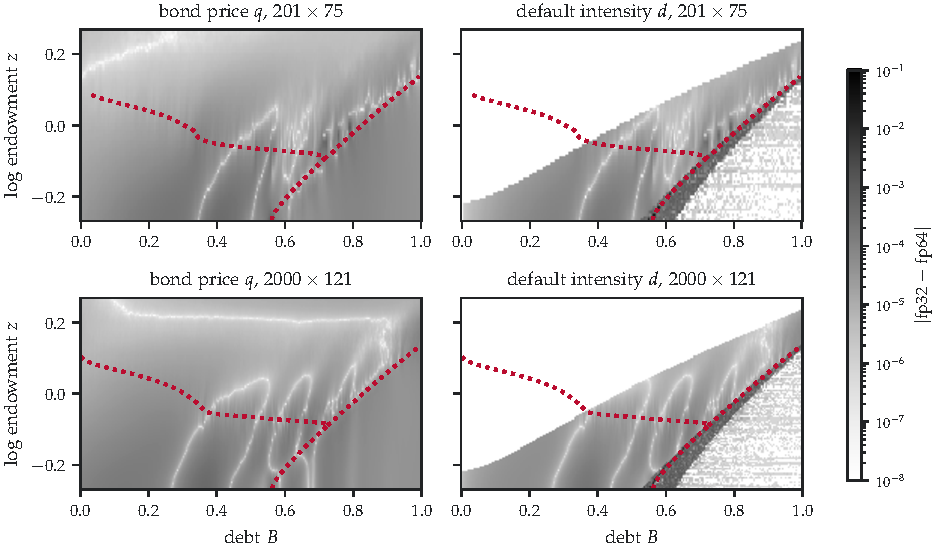
\includegraphics[width=\textwidth]{fp32_maps.pdf}
\caption{Absolute difference between the GPU \fps\ and the CPU \fpd\ solutions over the state space, log scale. Top: paper grid. Bottom: $2000\times121$. Dotted: the zero-drift locus.}
\label{fig:fp32}
\end{figure}

The \fps\ moments in Table~\ref{tab:table2} agree with \fpd\ to the reported digits. \fps\ is the faster precision on both back ends (Table~\ref{tab:times}): on the CPU it shortens the total by 5 to 40 percent, and on the GPU it is 4 to 6 times faster in total and 10 to 17 times faster in the solve. On this GPU it is the only precision in which the GPU beats the CPU.

\section{Dense grids}
\label{sec:dense}

\paragraph{The dense-grid algorithm.} The model is solved on three dense grids, all with 121 endowment levels:
\begin{itemize}
\item $500\times121$: the paper's algorithm and criteria, unchanged, from the paper's starting point interpolated to the grid.
\item $1000\times121$: from the $500\times121$ solution of the same configuration, interpolated bilinearly, with $\Delta t_{\max}=0.25$ and $\text{tol}_q=10^{-6}$.
\item $2000\times121$: from the $1000\times121$ solution of the same configuration, interpolated bilinearly, with $\Delta t_{\max}=0.125$ and $\text{tol}_q=10^{-6}$.
\end{itemize}
In all three, $\text{tol}_V=10^{-7}$, $\Delta t_0=0.015$, the growth factor is 1.02, and stickiness and freezing are as in the paper; the largest time step follows the rule $\Delta t_{\max}=\min(0.5,\,250\,h_B)$, with $h_B$ the debt step, which gives the paper's 0.5 on the paper grid and on the $500\times121$ grid. The two changes on the finer grids have a common cause. Where issuance is capped by the underwriting standard ($q\approx0.6$, $B\approx0.73$, $z\approx-0.07$), the drift of debt changes sign between adjacent nodes, and on a fine debt grid a large pseudo-time step lets the branch choice and the price feed back on each other from one step to the next: the price residual settles into a cycle of about 20 steps at a few nodes instead of decaying. Scaling the largest time step with the debt step keeps the ratio of the pseudo-time step to the debt step at or below its value on the $500\times121$ grid, where the paper's algorithm converges. The cycle that remains has an amplitude of about $3\times10^{-7}$ in the price, so the price tolerance is $10^{-6}$; a price difference of $10^{-6}$ is a spread difference of about $3\times10^{-7}$, or $0.003$ basis points. Continuation from the coarser grid starts the iteration close to the equilibrium, so that the early transient, in which most branch changes and frozen nodes arise, is short. Table~\ref{tab:conv} reports the steps, the criteria, and the final residuals of every run.

\begin{table}[htbp]
\centering
\caption{Convergence of every run}
\label{tab:conv}
\footnotesize
\resizebox{\textwidth}{!}{%
\begin{tabular}{@{}l r c c c c r l@{}}
\toprule
Configuration & Steps & $\Delta t_{\max}$ & Criterion $(\text{tol}_V, \text{tol}_q)$ & $r_V$ & $r_q$ & Frozen & Stop\\
\midrule
\tabinput tables/convergence.tex 
\bottomrule
\end{tabular}}
\par\smallskip\begin{minipage}{\textwidth}\footnotesize Notes: $r_V$, $r_q$: final residuals of the stationary equations, max norm. Criterion: the tolerances of \fpd\ runs; $64\varepsilon_{32}$: the \fps\ rule of Section~\ref{sec:criteria}. Stop: the rule that ended the run.
\end{minipage}
\end{table}

\paragraph{Results.} The equilibrium is stable under refinement. Figure~\ref{fig:grids} overlays the price, the default intensity, and the drift of debt at one standard deviation below and above the mean, and the ergodic density of the spread, on the paper grid and on the $500\times121$ and $2000\times121$ grids; the lines coincide except near the jump of the drift at the underwriting standard, which the finer grids resolve more sharply. Table~\ref{tab:dense} reports Table~2 on each grid: every moment agrees across grids to within one unit in the last reported digit, the size of the simulation noise, and the loss stays between 0.256 and 0.257. The finer grids concentrate more ergodic mass exactly at the underwriting standard, which shows as a spike in the density of the spread at $q=\underline q$.

\begin{figure}[htbp]
\centering
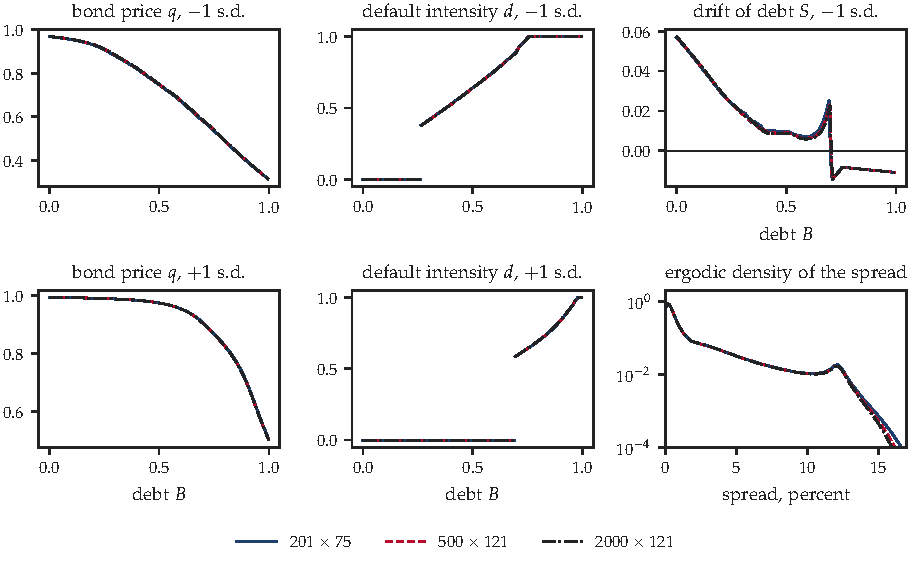
\includegraphics[width=\textwidth]{grid_slices.pdf}
\caption{The equilibrium on the paper grid and two dense grids (CPU, \fpd): bond price, default intensity, and drift of debt at one stationary standard deviation below and above the mean endowment, and the ergodic density of the spread, in percent, on a log scale.}
\label{fig:grids}
\end{figure}

\begin{table}[htbp]
\centering
\caption{Moments by grid (Table 2 of the paper)}
\label{tab:dense}
\footnotesize
\setlength{\tabcolsep}{3pt}
\resizebox{\textwidth}{!}{%
\begin{tabular}{@{}l c ccc c ccc@{}}
\toprule
& & & & & & \multicolumn{3}{c}{Dense grids}\\
\cmidrule(l){7-9}
& & & & & $201\times75$ & $500\times121$ & $1000\times121$ & $2000\times121$ \\
Moment & Weight & Data & AMR (2023) & This paper & CPU & CPU & CPU & CPU\\
\midrule
\tabinput tables/table2_dense.tex 
\bottomrule
\end{tabular}}
\par\smallskip\begin{minipage}{\textwidth}\footnotesize Notes: The rewrite in \fpd\ on the CPU on each grid. Data, AMR (2023), and This paper: Table~2 of the paper.
\end{minipage}
\end{table}

\section{Exhibits}
\label{sec:exhibits}

Figures~\ref{fig:slices201}--\ref{fig:states2000} reproduce Figures~6, 7, 8, and F.1 of the paper twice: from the rewrite's solution on the paper grid (CPU, \fpd), and from its converged solution on the $2000\times121$ grid (CPU, \fpd, with the ergodic density and the impulse responses computed on that grid). The figures are drawn by the plotting functions of the replication package (\texttt{code/make\_figures.py}), unchanged, from files in the package's layout written by \texttt{tools/plots.py}; on the dense grid the smoothing of the density and of the spread histogram, which the package sets in grid points, is rescaled to the same width in debt and in endowment units. The paper-grid figures are indistinguishable from those drawn from the package's stored solution, and the dense-grid figures differ only in the sharper resolution of the jumps at the default threshold and at the underwriting standard. In Figure~8 on the dense grid the spread rises on impact by 146 basis points (148 on the paper grid and in the paper), and debt peaks after ten years at 7.5 percent of mean output, as on the paper grid.

\newcommand{\exhibit}[4]{%
\begin{figure}[htbp]\centering
\includegraphics[width=\textwidth]{#1}
\caption{#2}\label{#3}
\end{figure}}

\exhibit{ou_slices_201.pdf}{Figure 6 of the paper, paper grid ($201\times75$): value, bond price, consumption, default intensity, and drift of debt as functions of debt at four endowment levels, one and two stationary standard deviations below and above the mean, and the ergodic density of the spread, in percent, on a log scale. Dotted: the spread at the underwriting standard.}{fig:slices201}{}
\exhibit{ou_slices_2000.pdf}{Figure 6 of the paper, $2000\times121$ grid. As in Figure~\ref{fig:slices201}.}{fig:slices2000}{}
\exhibit{ou_contours_201.pdf}{Figure 7 of the paper, paper grid: contours of the bond price, of the default intensity, and of the ergodic density. The density contours enclose 50, 75, 90, and 99 percent of the mass on positive debt. Dotted: the zero-drift locus, where debt is stationary.}{fig:contours201}{}
\exhibit{ou_contours_2000.pdf}{Figure 7 of the paper, $2000\times121$ grid. As in Figure~\ref{fig:contours201}.}{fig:contours2000}{}
\exhibit{ou_irf_201.pdf}{Figure 8 of the paper, paper grid: impulse responses to a negative shock of 0.1 to the log endowment at date zero, from the ergodic distribution: expected path under the forward equation minus the ergodic mean. Flows are in percent of mean annual output, and the spread is in basis points.}{fig:irf201}{}
\exhibit{ou_irf_2000.pdf}{Figure 8 of the paper, $2000\times121$ grid. As in Figure~\ref{fig:irf201}.}{fig:irf2000}{}
\exhibit{ou_irf_states_201.pdf}{Figure F.1 of the paper, paper grid: the same shock from three states. The economy is at the mean endowment with debt at its ergodic mean (solid), 25 percent below it (dashed), or 25 percent above it (dash-dotted): expected path under the forward equation from that state minus the path from the same state without the shock. The last panel shows arrears as a share of the gross additions to debt, new issues plus arrears, along the shocked path.}{fig:states201}{}
\exhibit{ou_irf_states_2000.pdf}{Figure F.1 of the paper, $2000\times121$ grid. As in Figure~\ref{fig:states201}.}{fig:states2000}{}

\clearpage
\appendix
\section{Code and reproduction}

\begin{tabular}{@{}>{\ttfamily}l p{0.68\textwidth}@{}}
\toprule
src/km.cu & driver: options, input, stage timing, output \\
src/model.h & model primitives, the node problem (three branches, golden-section search), Philox \\
src/shared.h & data structures and the simulation of one segment, shared by both back ends \\
src/cpu\_backend.h & CPU solve: policy step, line and block line Gauss--Seidel, stopping rules, simulation \\
src/gpu\_backend.cuh & GPU solve: policy, residual, factorization, extrapolation, and cooperative sweep kernels \\
src/post.h & ergodic density, ergodic and path moments, impulse responses (CPU and GPU), output \\
tools/make\_inputs.py & parameters and starting point from the replication package \\
tools/to\_init.py & a solution as the starting point of a finer grid (continuation) \\
tools/bench.sh & the runs of this report \\
tools/tables.py & the tables of this report \\
tools/plots.py & the exhibits, with the package's plotting functions \\
tools/plots\_extra.py & Figures~\ref{fig:fp32} and~\ref{fig:grids} \\
baseline/bench\_ref.py & the timed run of the paper's code on the paper grid \\
\bottomrule
\end{tabular}

\medskip
\noindent \texttt{make} builds \texttt{bin/km}; \texttt{tools/bench.sh} runs every configuration of the tables and writes \texttt{results/}; \texttt{python tools/tables.py} and \texttt{python tools/plots.py results/p\_cpu64 report/figures \_201} (and \texttt{results/d2000\_cpu64 \ldots\ \_2000}) remake the tables and figures. The README lists every option of \texttt{bin/km}.

\end{document}
